\documentclass[10pt]{exam}

\usepackage{amssymb, amsmath, amsthm, mathrsfs, multicol, graphicx}
\usepackage{tikz}

 \def\d{\displaystyle}
\def\?{\reflectbox{?}}
\def\b#1{\mathbf{#1}}
\def\f#1{\mathfrak #1}
\def\c#1{\mathcal #1}
\def\s#1{\mathscr #1}
\def\r#1{\mathrm{#1}}
\def\N{\mathbb N}
\def\Z{\mathbb Z}
\def\Q{\mathbb Q}
\def\R{\mathbb R}
\def\C{\mathbb C}
\def\F{\mathbb F}
\def\A{\mathbb A}
\def\X{\mathbb X}
\def\E{\mathbb E}
\def\O{\mathbb O}
\def\U{\mathcal U}
\def\pow{\mathcal P}
\def\inv{^{-1}}
\def\nrml{\triangleleft}
\def\st{:}
\def\~{\widetilde}
\def\rem{\mathcal R}
\def\sigalg{$\sigma$-algebra }
\def\Gal{\mbox{Gal}}
\def\iff{\leftrightarrow}
\def\Iff{\Leftrightarrow}
\def\land{\wedge}
\def\And{\bigwedge}
\def\AAnd{\d\bigwedge\mkern-18mu\bigwedge}
\def\Vee{\bigvee}
\def\VVee{\d\Vee\mkern-18mu\Vee}
\def\imp{\rightarrow}
\def\Imp{\Rightarrow}
\def\Fi{\Leftarrow}

%\def\={\equiv}
\def\var{\mbox{var}}
\def\mod{\mbox{Mod}}
\def\Th{\mbox{Th}}
\def\sat{\mbox{Sat}}
\def\con{\mbox{Con}}
\def\bmodels{=\joinrel\mathrel|}
\def\iffmodels{\bmodels\models}
\def\dbland{\bigwedge \!\!\bigwedge}
\def\dom{\mbox{dom}}
\def\rng{\mbox{range}}
\DeclareMathOperator{\wgt}{wgt}


\def\bar{\overline}


\newcommand{\vtx}[2]{node[fill,circle,inner sep=0pt, minimum size=4pt,label=#1:#2]{}}
\newcommand{\va}[1]{\vtx{above}{#1}}
\newcommand{\vb}[1]{\vtx{below}{#1}}
\newcommand{\vr}[1]{\vtx{right}{#1}}
\newcommand{\vl}[1]{\vtx{left}{#1}}
\renewcommand{\v}{\vtx{above}{}}

\def\circleA{(-.5,0) circle (1)}
\def\circleAlabel{(-1.5,.6) node[above]{$A$}}
\def\circleB{(.5,0) circle (1)}
\def\circleBlabel{(1.5,.6) node[above]{$B$}}
\def\circleC{(0,-1) circle (1)}
\def\circleClabel{(.5,-2) node[right]{$C$}}
\def\twosetbox{(-2,-1.4) rectangle (2,1.4)}
\def\threesetbox{(-2.5,-2.4) rectangle (2.5,1.4)}
\newcommand{\twoline}[2]{\begin{pmatrix}#1 \\ #2 \end{pmatrix}}


\def\circleA{(-.5,0) circle (1)}
\def\circleAlabel{(-1.5,.6) node[above]{$A$}}
\def\circleB{(.5,0) circle (1)}
\def\circleBlabel{(1.5,.6) node[above]{$B$}}
\def\circleC{(0,-1) circle (1)}
\def\circleClabel{(.5,-2) node[right]{$C$}}
\def\twosetbox{(-2,-1.5) rectangle (2,1.5)}
\def\threesetbox{(-2,-2.5) rectangle (2,1.5)}

%\pointname{pts}
\pointsinmargin
\marginpointname{pts}
\bonuspointname{pts}
\marginbonuspointname{pts}
\addpoints
\pagestyle{head}
%\printanswers

\firstpageheader{Math 228}{\bf Homework 9}{Due: Wednesday, November 8}


\begin{document}
\noindent \textbf{Instructions}: Same rules as usual -- turn in your work on separate sheets of paper.  You must justify all your answers for full credit.  Do not consult the Internet.

\begin{questions}

  \question[9] Suppose that you would like to prove the following implication:
  \begin{center}
  ``For all numbers $n$, if $n$ is prime then $n$ is solitary.''
  \end{center}
  Write out the beginning and end of the argument if you were to prove the statement,
  \begin{parts}
  \part Directly
  \begin{solution}
  To prove the above statement using a direct proof we would need to start by  assuming that $n$ is a prime number then using logic, logic, logic,... we could conclude that $n$ is solitary.
  \end{solution}
  \part By contrapositive
  \begin{solution}
  To prove by contrapositive: Assume $n$ is not solitary (logic, logic, logic...) and conclude that $n$ is not prime.
  \end{solution}
  \part By contradiction
  \begin{solution}
  To prove using a proof by contradiction: Assume that $n$ is prime and that $n$ is not solitary (logic, logic, logic...) then either $n$ is not prime or $n$ is solitary (you need to contradict one of your assumptions). Therefore, if $n$ is prime then $n$ is solitary.
  \end{solution}
  \end{parts}
  You do not need to provide details for the proofs (since you do not know what solitary means). However, make sure that you provide the first few and last few lines of the proofs so that we can see that logical structure you would follow.



  \question[9] A standard deck of 52 cards consists of 4 suites (hearts, diamonds, spades and clubs) each containing 13 different values (Ace, 2, 3, \ldots, 10, J, Q, K).  If you draw some number of cards at random you might or might not have a pair (two cards with the same value) or three cards all of the same suit.  However, if you draw enough cards, you will be guaranteed to have these.  For each of the following, find the smallest number of cards you would need to draw to be guaranteed having the specified cards.  \underline{Prove your answers} (and specify what sort of proof you are using).
  \begin{parts}
  \part Three of a kind (for example, three 7's).
  \begin{solution}
  The smallest number of cards you must draw is 27.  If you drew 26, you could have two of each value, and as such not have three of a kind.  To prove that 27 cards guarantees a three of a kind, we give a proof by contrapositive.

  Suppose you do not have a three of a kind.  Then you have at most two of each value, so at most 26 cards.  Thus you do not have 27 cards.

  \end{solution}
  \part A flush of five cards (for example, five hearts).
  \begin{solution}
    The smallest number of cards needed is 17.  If you had 16 cards, you could have 4 of each suit.  In fact, if you did not have a flush of five cards, you could have at most 4 of each suit, for only 16 cards.  Thus you don't have 17 cards.

  \end{solution}
  \part Three cards that are either all the same suit or all different suits.
  \begin{solution}
  You must pick 5 cards.  If you picked just 4, you could have two hearts and two spades.  However, given any 5 cards, we can be sure that at least two of them will be the same suit, say hearts.  Of the remaining three cards, if any of them are also a heart, we will have three hearts.  If not,  there are two cases to consider.  Either all three cards will be of the same suit (in which case we would have three cards of the same suit) or else two suits will be present among the three cards.  But those two other suits are not hearts, so those two cards plus one of the hearts will form a set of three cards of all different suits.

  An alternative proof: suppose you did not have three cards all the same or all different.  Then you can have at most two cards of any given suit, and at most two suits.  This is at most 4 cards.
  \end{solution}
  \end{parts}



  \question[6] Suppose you are at a party with 19 of your closest friends (so including you, there are 20 people there).  Explain why there must be least two people at the party who are friends with the same number of people at the party.  Assume friendship is always reciprocated.

  \begin{solution}
    Suppose this was not the case.  That is, suppose everyone at the party had a {\em different} number of friends.  What could these numbers be.  Any give person at the party could have between 0 and 19 friends at the party.  This is 20 numbers, but we can't have all of these numbers occur at the same party.  If someone is friends with 19 people, then she is friends with everyone, including the person who is supposedly friends with 0 people.  Thus there are only 19 values for the number of friends people can have, so two people must have the same number of friends.

    What this says is that in any graph with 20 vertices, there must be at least two vertices which have the same degree.
  \end{solution}


  \question[6] Consider the following two graphs:\\
  $G_1$: $V_1=\{a,b,c,d,e,f,g\}$, $E_1=\{\{a,b\},\{a,d\},\{b,c\},\{b,d\},\{b,e\},\{b,f\},\{c,g\},\{d,e\},\{e,f\},\{f,g\}\}$.\\
  $G_2$: $V_2=\{v_1,v_2,v_3,v_4,v_5,v_6,v_7\}$,

  \hspace{1.75em} $E_2=\{\{v_1,v_4\},\{v_1,v_5\},\{v_1,v_7\},\{v_2,v_3\},\{v_2,v_6\},\{v_3,v_5\},\{v_3,v_7\},\{v_4,v_5\},\{v_5,v_6\},\{v_5,v_7\}\}$.
  \begin{parts}
  \part Let $f:G_1 \rightarrow G_2$ be a function that takes the vertices of Graph 1 to vertices of Graph 2.  The function is given by the following table:

  \begin{center}
  \begin{tabular}{c*{7}{|c}}
  $x$ & $a$ & $b$ & $c$ & $d$ & $e$ & $f$ & $g$ \\ \hline
  $f(x)$ & $v_4$ & $v_5$ & $v_1$ & $v_6$ & $v_2$ & $v_3$ & $v_7$
  \end{tabular}
  \end{center}
  %
  %\[f(a)=v_4\]
  %\[f(b)=v_5\]
  %\[f(c)=v_1\]
  %\[f(d)=v_6\]
  %\[f(e)=v_2\]
  %\[f(f)=v_3\]
  %\[f(g)=v_7\]
  Is $f$ an isomorphism between Graph 1 and Graph 2? Explain.
  \begin{solution}
  Recall that in order for $f$ to be an isomorphism between $G1$ and $G2$, it must preserve relationships between vertices. To put this into context, this means that since $a$ and $b$ are joined via an edge in $G1$ that their corresponding vertices in $G2$ must also be joined by an edge. This must be true for all of the vertices and edges. When examining the function, we can see that the vertex $g$ goes to $v_7$, that is $f(g)=v_7$. BUT, $g$ has exactly 2 edges (so $g$ is degree 2) and $v_7$ is degree 3. This means that $f$ cannot possibly be an isomorphism. Similarly, we can see that $f$ does not take $c$ to the correct vertex either $c$ is degree 2 and $v_1$ has degree 3.
  \end{solution}
  \part Define a function $g$ (different from $f$) that \emph{is} an isomorphism between Graph 1 and Graph 2.
  \begin{solution}
  \begin{center}
  \begin{tabular}{c*{7}{|c}}
  $x$ & $a$ & $b$ & $c$ & $d$ & $e$ & $f$ & $g$ \\ \hline
  $g(x)$ & $v_4$ & $v_5$ & $v_6$ & $v_1$ & $v_7$ & $v_3$ & $v_2$
  \end{tabular}
  \end{center}
  \end{solution}
  \part Is the graph pictured below isomorphic to Graph 1 and Graph 2? Explain.
  \begin{center}
  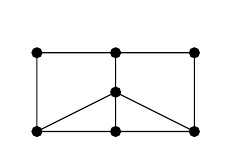
\begin{tikzpicture}
  \draw (-1, 0) coordinate (v1) -- (0,0) coordinate (v2) -- (1,0) coordinate (v3) -- (1,1) coordinate (v4) -- (0,1) coordinate (v5) -- (-1,1) coordinate (v6) -- (v1) --(0,.5) coordinate (v7) -- (v2) (v7) -- (v3) (v7) -- (v5);
  \foreach \i in {1,...,7}{
  	\fill (v\i) \v;
  }
  \end{tikzpicture}
  \begin{solution}
  No, it could not possibly be isomorphic. If you count up the degrees of each vertex in this picture, you can see that the highest degree is 4 (the center vertex). In order to be isomorphic to either $G1$ or $G2$ we would definitely need a vertex of degree 5, which we don't have.
  \end{solution}

  \end{center}

  \end{parts}


  \bonusquestion[4] Bonus: Suppose a $n\times n$ chessboard is missing two opposite corners.  Prove that no matter what $n$ is, you will not be able to cover the remaining squares exactly with dominoes.

  \begin{center}
  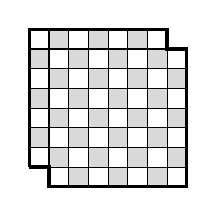
\begin{tikzpicture}[scale=.25]
  \foreach \x in {0,2,...,6}{
  	\foreach \y in {0,2,...,6}{
  \draw[fill=white!85!black] (\x,\y) rectangle (\x+1, \y+1) rectangle (\x+2,\y+2);
  }}
  \draw (0,0) grid (8,8);
  \draw[white, fill=white] (7,7) rectangle (8,8) (0,0) rectangle (1,1);
  \draw[very thick] (0,1) -- (1,1) -- (1,0) -- (8,0) --(8,7) -- (7,7) -- (7,8) -- (0,8) -- (0,1);
  \end{tikzpicture}
  \end{center}

  \begin{solution}
  If $n$ is odd, then $n^2$ is odd, as is $n^2 - 2$.  Thus it would be impossible to cover the board with dominoes.  If $n$ is even, then this is not an issue any more.  However, notice that the opposite squares are the same color, so removing them would result in more squares of one color than the other.  Every domino needs to cover two adjacent squares, so one square of each color.  Thus any attempt two cover the board with dominoes will result in two uncovered squares (of the color you have more of).
  \end{solution}
\end{questions}
\end{document}
